\documentclass[twocolumn]{article}
\usepackage{amsmath}
\usepackage{xtab}
\usepackage{graphicx}
\usepackage{subfigure}
\usepackage{fullpage}
\usepackage{blindtext}   %Texto de relleno
\usepackage{hyperref}

\author{Marcela De La Cruz}
\date{4 de Julio de 2016}


\title{\sc Ecuaciones, tablas y figuras}
\pagestyle{empty}

\begin{document}
\maketitle	
\thispagestyle{empty}
\section{Figuras} % (fold)
\label{sec:Figuras}


\blindtext

En la figura \ref{fig:ciencia} podemos apreciar un collage con t\'erminos matem\'aticos, en la figura \ref{fig:mus y mat} se muestra una imagen que hace referencia a la relaci\'on que existe entre la m\'usica y las matem\'aticas.


\begin{figure}[h]
	\centering
	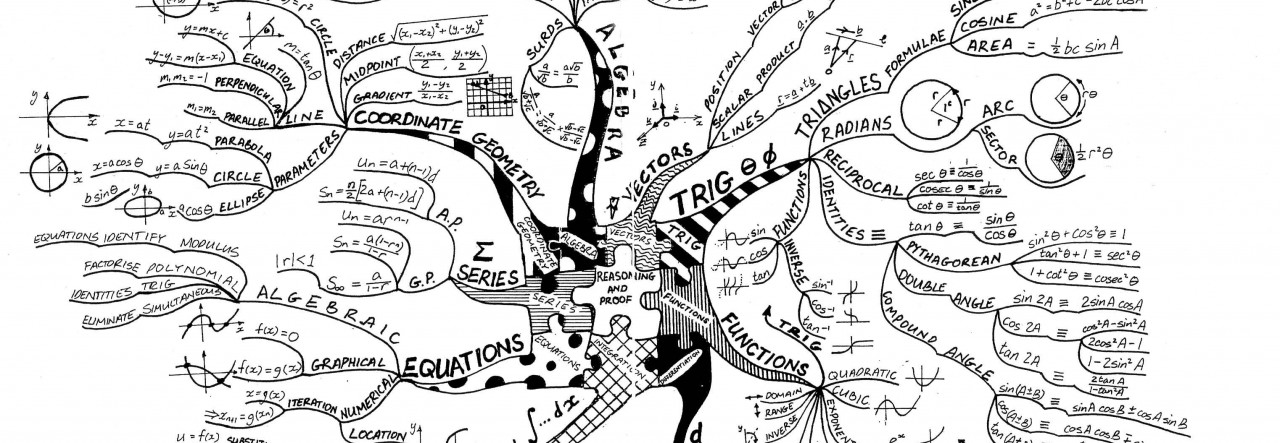
\includegraphics[width=0.5\textwidth]{imagen1}
	\caption{Matem\'aticas}
	\label{fig:ciencia}
\end{figure}


\begin{figure}[h]
	\centering
	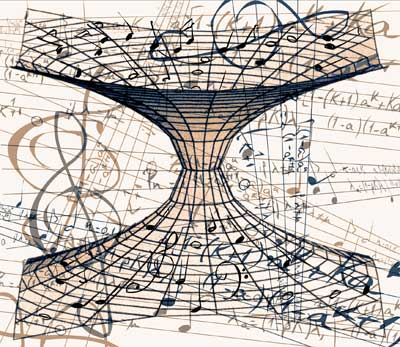
\includegraphics[width=0.5\textwidth]{musica-matematicas}
	\caption{La m\'usica y las matem\'aticas}
	\label{fig:mus y mat}
\end{figure}

Para m\'as informaci\'on revisar  \href{https://en.wikibooks.org/wiki/LaTeX/Floats,_Figures_and_Captions}{este v\'inculo}

% section figuras (end)
\section{Ecuaciones} % (fold)
\label{sec:ecuaciones}

Como se vi\'o en la secci\'on \ref{sec:Figuras} se pueden citar distintos v\'inculos


% section ecuaciones (end)

\section{Tablas} % (fold)
\label{sec:Tablas}
\begin{center}
	

\begin{tabular}{|l|c|l|}

\hline
\textbf{Nombre} & \textbf{Edad} & \textbf{Estado} \\
\hline	
\hline	

Reinaldo   &  32  &  Guanajuato \\
Marcela    &  21  &  Tabasco \\
Ana & 24 & Tabasco \\
Guillermo  &  24  &  Quer\'etaro \\

\hline

\end{tabular}
\end{center}



% section section_name (end)






\end{document}
\maketitle	